\documentclass{../industrial-development}
\graphicspath{{5-organization-of-developer-work/}}

\title{Методы и техники организации работы разработчика}
\author{Заплатин Егор Сергеевич, ПИ-21 МО}
\date{}

\begin{document}

\begin{frame}
  \titlepage
\end{frame}

\section{Управление задачами}

\subsection{Разбиение задач на категории}

\begin{frame} \frametitle{Разбиение задач на категории}

  \begin{itemize}
  \item Когда задач становиться много сложно понять за что взяться в первую очередь
  \item Приницип, стоящий в основе управление задачами --- составление списка задач
  \item Задачи нужно разбивать на категории по какому-то принципу, например по важности
  \end{itemize}
\end{frame}

\lecturenotes

Когда только начинаешь работать, то все ясно и понятно, задач не так много, есть представление как с ними работать. Но со временем приходит осознание, что задач накопилось очень много.

Принцип, который необходимо положить в основу — составление списка задач. Посмотрите на свои задачи и проставьте у каждой приоритет и сколько вы думаете затрать на нее времени. Если у вас слишком много задач, то подумайте, по какому критерию вы можете сократить рассматриваемый список задач. Например, вы можете отобрать только задачи в ближайшую версию исправления, только задачи в текущий спринт (если вы работаете по Scrum) и так далее. И именно с этим списком и стоит работать.

Итак, все дела списка разделите на 4 группы:
\begin{itemize}
\item Срочные и важные
\item Важные, но не срочные
\item Срочные, но неважные
\item Не срочные и неважные~\cite{TMHabr}
\end{itemize}

\begin{frame} \frametitle{Схема централизованного контроля версий}
  \centerline{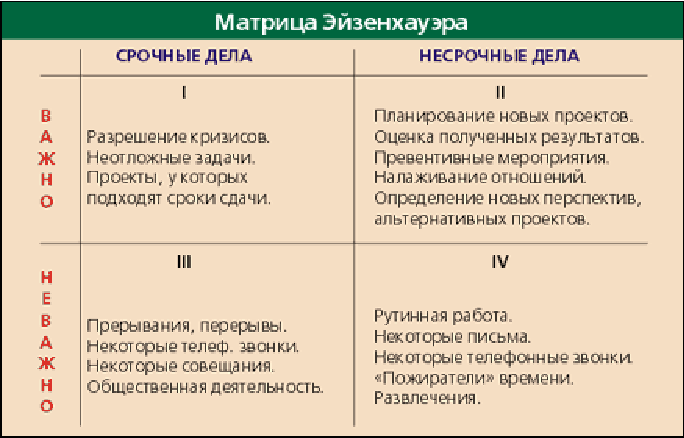
\includegraphics[width=0.8\textwidth]{EisenhowMeratrix.pdf}}
\end{frame}

\begin{frame} \frametitle{Правила работы с задачами}
  \begin{itemize}
  \item У каждой задачи проставляется время на её решение
  \item Шаг планирования ровно один рабочий день
  \item Время отдыха также стоит планировать
  \item Помимо важных и долгих нужны лёгкие и быстрые задачи для того, чтобы была возможность расслабиться
  \item У каждой задачи если лимит времени на решение
  \item Стоит составлять список минимум и список максимум
  \item Список должен быть где-то зафиксирован
  \item Время на форс-мажоры тоже должно быть запланировано
  \end{itemize}
\end{frame}

\lecturenotes

Теперь у каждой задачи проставим время, которое мы потратим на ее решение. И, помня, что у нас всего 8 рабочих часов в день, составим список задач на сегодня. Список стоит составлять накануне вечером либо как только вы придете на работу.

Очень важно, что все задачи вы должны планировать исходя из того, чтобы сделать их ровно в рабочий день. Никак не больше. Не планируйте работать сверхурочно без крайней необходимости. Это приведет только к усталости. Лучше потратить свободное время на саморазвитие и чтение профессиональной литературы.

Не забудьте учесть, что у вас чистых рабочих меньше, чем 8 часов. Нужно учесть время на перерывы, отдых физический. Разработчик не должен все время сидеть за компьютером. Запланируйте, что хотя бы по 15 минут каждые два часа вы будете выгонять себя, вставать и просто пройдетесь и проветритесь. При этом эффективность работы только вырастет. Это поможет, не теряя темпа, успеть сделать то, что не смог бы сделать без отдыха.
НО, не нужно злоупотреблять. На перерыв можно потратить максимум полчаса, иначе мозг слишком расслабляется и теряется рабочий настрой.

В этом списке должны быть не только важные и долгие задачи, но и лёгкие, быстрые, чтобы на них можно было переключить внимание, расслабиться. Для разработчика это крайне важно. Задачи можно выполнять в любом порядке, но тем не менее рекомендуется начинать с важных. И обязательно начать с тех, которые меньше всего хочется делать.

Установите лимит времени на решение задачи. Если вы безрезультатно (именно безрезультатно!) сидите над задачей больше 2 часов, то пришла пора переключиться на другую задачу. У вас в списке есть такие задачи в разряде простых. Мы их специально для этого и включили.

Составьте список минимум и список максимум. Список минимум должен быть выполнен обязательно. К тому же при его выполнении вы почувствуете удовлетворенность собой. Список максимум нужен, если останется время. Если вы не успели свою программу минимум, то вы неправильно оцениваете свои силы, нужно подходить к этому более тщательно.
Если вы научились выполнять список минимум и у вас уже который день подряд остается время на список максимум, то пора увеличивать список минимум. И да, опять же — снова смотреть почему вы неправильно оценили время на задачи.

Зафиксируйте где-то список: на бумаге или в электронной версии. Но так, чтобы он был у вас перед глазами. Это поможет видеть сколько уже сделано и сколько еще осталось. Также вы получите эмоциональное удовлетворение при вычеркивании очередной задачи из списка, а это даст дополнительную мотивацию. Поэтому очень важно именно вычеркивать задачи, а не удалять.

Запланируйте время на форс-мажоры. Как гласит закон Мёрфи «если что-то может случиться, то это обязательно случится». Как правило, разработчики чувствуют такие моменты~\cite{TMHabr}.

\begin{frame} \frametitle{Работа с тяжёлыми задачами}
  \begin{itemize}
  \item Неподъемная задача должна стоять первой в списке
  \item Если появлось желание отложить задачу на завтра, это знак, что ей нужно заняться прямо сейчас
  \item Можно представлять себе, что осталась только одна эта тяжёлая задача
  \item Если нужна концентрация стоит включить «турбо режим»
  \end{itemize}
\end{frame}

\lecturenotes

Рассмотрим работу с тяжелыми задачами. Теми, которые почему-то кажутся неподъемными. Они пугают либо тем, что непонятно как к такой задаче подступиться, либо тем, что не хочется общаться с ее автором/заказчиком. Следующие несколько правил именно о таких задачах.

Если у вас появилась неподъемная задача, за которую вы не хотите приниматься или не знаете как оценить, то она должна встать первой в вашем списке. Это потенциальная черная дыра и может оказаться неразрешимой для вас или слишком затратной по времени, что грозит тем, что вы ее просто не успеете сделать. Начните с нее, возвращайтесь к ней в течение дня, пока она не станет для вас понятной, попробуйте разбить ее на более мелкие. 
Также может помочь просто рассказать кому-то из коллег о задаче, отобразить ее на доске или даже просто рассказать вслух о проблеме.
Как только хочется отложить задачу на завтра, то это знак, чтобы заняться ей прямо сейчас.

Старайтесь выполнить задачи так, чтобы если у вас и осталась эта неподъемная задача, то только она одна. Иначе у вас не будет удовлетворения и будет зависание на одной этой задаче и ряд невыполненных других.

Если вам нужна концентрация, используйте турбо-режим. Он действительно работает. Для этого на определенное время отключите все средства связи (skype, icq и др.), поставьте табличку, чтобы вас не отвлекали, оденьте наушники и не реагируйте ни на что. В эти 25 минут вы занимаетесь только решением одной конкретной задачи. Не отвлекайтесь ни на что. Главное не злоупотреблять этим, особенно в крупных компаниях~\cite{TMHabr}.

\subsection{Разбиение задач на подзадачи}

\begin{frame} \frametitle{Разбиение задач на подзадачи}
  \begin{itemize}
  \item Множество задач, нужно раздробить на понятные целые единицы работы
  \item Разбиение на подзадачи позволяет отслеживать прогресс
  \item Каждая небольшая решённая задача — это успех, который мотивирует
  \item Инструменты визуализации и планирования вроде досок и заметок помогают видеть действительно выполненную работу и потраченное время
  \end{itemize}
\end{frame}

\lecturenotes

Когда мы подходим к чему-то со всей серьёзностью, когда мы работаем с большим количеством людей, мы должны тщательно спланировать каждый свой шаг. Это поможет избежать ошибок, видеть свой прогресс и отслеживать реализацию.
Это касается и основных трудовых задач.К примеру, нужно разбить приложение на модули, отделить графический интерфейс от бэкенда. И работать над каждым модулем отдельно.
Каждый модуль разбивается на конкретные задачи.
И даже это множество задач, нужно раздробить на понятные целые единицы работы. Зачем? Чтобы не получилось нечто ужасное.
Эту задачу изначально нужно было разбить на подзадачи, чтобы видеть прогресс. Я имею ввиду, что каждая небольшая решённая задача — это успех, который мотивирует. А огромная задача, прогресс которой невозможно отследить в течение 2-х дней — это подавляющая стремления проблема.
Я проделал огромную работу, но результат своих трудов увидел только в конце задачи. Это очень утомляет, когда не видишь успех, когда не можешь выделить конкретные решённые вопросы.
Всегда разбивайте задачи на подзадачи. Смотрите за своим прогрессом и мотивируйте себя им. Используйте различные инструменты планирования, вроде досок и заметок. Это поможет вам видеть свою действительно выполненную работу и потраченное время. А в дальнейшем это поможет вам “на лету” оценивать задачи~\cite{TasksMedium}.

\begin{frame} \frametitle{Как сделать, чтобы разбиение на подзадачи работало}
  \begin{itemize}
  \item Когда вы ставите короткую задачу, она не должна быть 100\% предсказанной
  \item Важно или не отвлекаться от выполнения модели предсказания
  \item Короткие мотивационные задачи не должны превышать 3 суток, а лучше всего максимум несколько часов, и обязательно должны подтверждаться фактом их достижения
  \end{itemize}
\end{frame}

\lecturenotes

Основной механизм функционирования человека в нашей сложной системе поведения, это умение предсказывать (модели предсказания, созданные нашим опытом). 

Возможность предсказывать лежит в основе создания коротких целей. Однако не всё так просто.
Если мы создаем предсказание с максимальной вероятностью (100\%), то оно не создает позитивной мотивации.
Мотивация же относится к тем случаям, когда предсказание не гарантирует достижение цели, но мы своими усилиями, на основе предсказания, всё же достигаем позитивного результата. Притом сила мотивации пропорциональна соотношению двух факторов: «бонус» и вероятность.
Точно также действуют и короткие задачи.

Когда вы ставите короткую задачу, она не должна быть 100\% предсказанной, то есть вы не должны детально четко знать каждый шаг по ее достижению. Это снижает «бонус», которым нас мотивирует подсознание. Если вы будете это знать, то такое задание не вызывает позитива, но является растратой ресурсов, так создается «рутина».

Если вы ставите короткую задачу средней предсказанности и реализуете ее точно со своей моделью предсказания, вы получаете свой позитив.

Собственно почему тогда задачи нужны именно короткие?

Дело в том, что поставив цель, вы создаете предсказание ее достижения, и подсознание по умолчанию считает, что в реализацию предсказания входят все действия между ее постановкой и окончательным результатом.

Если вы предсказываете, что сделаете модуль за 30 минут, подсознание дает мотивацию на достижение, так как считает, что вы будете непрерывно заниматься этим модулем и имеете вероятность его закончить именно через 30 минут.
Если же каждые 5 минут вас начинают «дергать», то подсознание может в результате понизить мотивацию, как эти «дерганья» начинают включаться в модель предсказания, и тем самым ваш модуль «стОит» для подсознания уже гораздо дороже, а такую цену оно возможно не готово платить.

Если такие случаи будут повторяться, то подсознание вырабатывает уже новое предсказание, которое не способно вас будет замотировать даже на этот простой модуль.

Именно поэтому в таких случаях важно или не отвлекаться от выполнения модели предсказания, или уметь очень сильно и четко переключать своё сознание, чтобы также и переключалось предсказание. Это довольно сложно сделать, если вас переключают на другие дела, требующие умственных усилий, но гораздо легче, если эти переключения идут в область 100\% предсказаний, например отлучиться в туалет.

Всё это гораздо сложнее реализовать для больших задач, следовательно на большие задачи требуются более сложные методы мотивации и конечно разбиение их на подзадачи.

В идеале короткие мотивационные задачи не должны превышать 3 суток, а лучше всего максимум несколько часов, и обязательно должны подтверждаться фактом их достижения, чтобы подсознание фиксировало, что предсказание успешно завершено~\cite{TasksHabr}.

\section{Управление рабочим временем}

\subsection{Принципы тайм-менеджмета для разработчика}

\begin{frame} \frametitle{Принципы тайм-менеджмета для разработчика}
  \begin{itemize}
  \item Отслеживать все задачи, вести журнал задач
  \item Делегировать задачи, когда это возможно
  \item Идеально не лучше, чем хорошо
  \item Надо найти время когда количество отвлечений будет минимально
  \item Необходимо планировать время на расслабление и отдых
  \item Награди себя
  \end{itemize}
\end{frame}

\lecturenotes

Если вы ничего не планируете сейчас, не беспокойтесь, вы можете это сделать позже. Просто отследите, что вы делаете на бумаге, листе Excel или используете программное обеспечение для управления задачами. Обновляйте список каждые два часа или, по крайней мере, в конце дня в начале. Это поможет вам найти общие прерыватели и повторяющиеся задачи, таким образом, вы сможете планировать вещи на будущее. Даже одна неделя дневного отслеживания может рассказать о том, как мы живем.
Посмотрите на свой журнал времени и попытайтесь выяснить, что действительно не нужно делать, что может сделать кто-то другой, работу, которую можно сделать более эффективно или быстро, действия, которые тратят время других и т. Д.

Делегировать задачи, когда это возможно
Если кто-то, кто может принять участие в вашей работе, не стесняйтесь поделиться с ним некоторой работой. Опишите задачу четко.
В многопроектной среде работа всей команды не может быть распределена поровну каждому члену. Кому-то придется делать больше и кого-то меньше. Используя теорию ограничений Голдрата, проект не может быть завершен до тех пор, пока самый медленный член не завершит свою работу. Таким образом, делегацию следует продвигать внутри команды, причем не только от менеджера до разработчика. Этот процесс может быть эффективен только в командах с честным и открытым общением.

Идеально не лучше, чем хорошо.
Например, при написании кода важно закончить вовремя, чем беспокоиться о идеальном решении, которое подходит для всех. Завершите работу, дополнительные функции можно добавить позже.  Исползуйте модульные тесты, это может улучшить качество и ускорить разработку.

Определите свое время
Человек - это социальное существо, мы имеем дело с людьми каждый день и час. У нас есть коллеги, друзья или родственники. Они могут помогать или замедлять вас различными способами. Кто-то может спросить вас напрямую, по телефону, через месенджер или по электронной почте. Это приводит к прерываниям, а также затратам времени. Прерывание в течение 6 -- 9 минут обычно требует дополнительных 4 -- 5 минут для восстановления. Пять перрываний будут стоит в час. Всегда хорошо думать о способах уменьшить частоту таких перерывов. Единственный способ сократить такие затраты времени - найти повторяющиеся отходы времени. Как только вы получите всю картину, легко решить, где сэкономить и где потратить.

Планирование расслабление и отдыха
Не ожидайте высокой производительности, если вы устали. Сон заряжает наши мозги и помогает нам мыслить более четко. Планируйте свой день адекватно, не забывайте спать.

Разработчики обычно сидят 8 часов в день или более на рабочем месте рядом с компьютером. Это приводит к эмоциональным и физическим заболеваниям. Один из наших уязвимых органов --- это глаза. Работа за монитором в течение длительного времени разрушает наше зрение. Чтобы уменьшить пагубное влияние на глаза, существует много методов тренировки глаз. Запланируйте его ежедневно, перед ужином или в любое другое удобное время.

Награди себя
Каждый ожидает награду или похвалу за свою работу, особенно за то, что он что-то законичил. Отсутствие награды может убить наше желание работать. Это обычно приводит к снижению производительности. Вот почему мы предпочитаем работать на других, чем делать что-то для себя. Обещайте себе награду после выполнения задания или завершения работы. Например, позвольте себе посмотреть интересный фильм, как только вы закончите разработку страницы или новой функции, или съешьте сладости или что-нибудь еще~\cite{TMCodeProject}.

\subsection{Персональные спринты}

\begin{frame} \frametitle{Персональные спринты}
  \begin{itemize}
  \item Можно применять технику «спринт» из Agile
  \item Несколько 45-минутных спринтов в день
  \item Сообщить своей команде, чтобы вас в это время не отвлекали
  \end{itemize}
\end{frame}

\lecturenotes

Многие команды разработчиков в наши дни слышали об Agile и, скорее всего, о том, что такое «спринт». Поэтому для большинства людей эта концепция должна быть хорошо известна. Как мы применим это к нашему личному времени работы?

Легко! Планируйте это. Начните в определенное время с определенной работы. И просто работайте над какой-то конкретной задачей. Это может быть несколько 45-минутных блоков. Но планируйте свой день для работы над конкретными задачами в определенное время, а затем выполняйте эту деятельность и минимизируйте прерывания в вашем спринте.

Сообщайте своей команде, что вы находитесь в процессе «персонального спринта», чтобы люди научились не прерывать вас, пока вы пытаетесь достичь состояния потока~\cite{TMSeimer}.

\subsection{Техника Pomodoro}

\begin{frame} \frametitle{Техника Pomodoro}
  \begin{itemize}
  \item Используем таймер для запланировнных действий
  \item Время одной Pomodoro стоит подбирать для себя
  \item Мелкие задачи стоит группировать
  \item Крупные задачи стиот разбивать на мелкие
  \item Чем больше применятеся эта техника, тем точнее можно планировать время
  \item Игнорируем отвлечения в процесе сеанаса Pomodoro
  \end{itemize}
\end{frame}

\lecturenotes

Несколько правил техники «Pomodoro» в тайм менеджменте:
\begin{itemize}
\item Использовать таймер для запланированных действий
\item Просматривайте временные затраты, чтобы лучше оценивать в будущем
\item Игнорируйте попытки отвлечения внимания во время сеансов Pomodoro~\cite{TMSeimer}
\item Известно, что продуктивность у всех людей разная, так же как и способность к концентрации, поэтому временные рамки при выполнении техники могут немного сдвигаться в ту или другую сторону. Например, кто-то может легко работать, не отвлекаясь, в течение 45 минут, тогда его «помидор» будет равняться именно этому времени. А кому-то 5 минут отдыха совсем не хватает, чтобы «перезагрузиться, тогда он может для себя установить 10-15 минутные перерывы
\item Если у вас есть задачи, на выполнение которых потребуется всего несколько минут, сгруппируйте их вместе в один «помидор», чтобы за 25 минут можно было решить все эти мелкие вопросы
\item И, наоборот, если на выполнение какого-то задания вам не хватит пяти 25-минуток, тогда следует разделить его на более мелкие задачи
\item Сам «помидор» делить на части запрещается, и прерываться во время «съедания помидора» тоже нельзя. Если вы вынужденно прервались более чем на минуту, перезапустите свой таймер и начните отсчет времени сначала~\cite{Pomidoro}
\end{itemize}

\begin{frame} \frametitle{Этапы техники Pomodoro}
  \begin{itemize}
  \item Постановка конкретной задачи
  \item Подготовка подручных средств: блокнот, ручку и таймер
  \item Установка таймера на 25-45 минут
  \item Непрерывная работа в течение 25 минут
  \item Перерыв на 5 минут
  \item Делаем ещё 3 помидора с пятиминутными перерывами
  \item Перерыв на 15-30 минут
  \end{itemize}
\end{frame}

\lecturenotes

Основные этапы работы по «методу помидора»:
\begin{enumerate}
  \item Постановка конкретной задачи, которой вы планируйте заняться непременно сегодня. В идеале, вы должны постоянно ставить перед собой цели и определять примерное время, в течение которого они будут достигнуты. А чтобы этого добиться, нужно определять еще задачи,  выполнение которые приведет вас к желаемым целям.  Совокупность таких задач – это ваш план на день
  \item Подготовка подручных средств, к которым отнесем блокнот, ручку и таймер (или будильник). Это самое простое, что всегда находится под рукой. Для более «продвинутых» можно посоветовать воспользоваться компьютерными программами, разработанными специально для управления временем по технике «помидор»
  \item Установка таймера на 25 минут. Считается, что это оптимальное время, чтобы сконцентрироваться на конкретной проблеме и, удерживая внимание, продуктивно над ней поработать без потери концентрации
  \item Непрерывная работа в течение 25 минут. Пока не раздастся сигнал таймера, свидетельствующий об окончании деятельности, вы должны сделать все, чтобы не отвлекаться на телефонные звонки, Интернет, проверку своего электронного ящика и соцсетей (Читайте «Хронофаги - поглотители и пожиратели рабочего времени»)
  \item Перерыв на 5 минут. Поставив галочку о завершении сессии, полностью отвлекитесь от работы, переключившись на другой вид деятельности, непременно расслабляющий
  \item Непрерывная работа в течение очередных 25 минут. Каждая такая 25-минутная работа называется помидором. Проделанная работа в течение этого времени = 1 помидор, который вы «съели»
  \item Второй перерыв на 5 минут
  \item Третий «помидор» на 25 минут
  \item Третий перерыв на 5 минут
  \item Четвертый «помидор» на 25 минут
  \item Перерыв на 15-30 минут. После такой трудоемкой деятельности непременно нужно сделать более продолжительный перерыв. 15-30 минут – это оптимальное время для отдыха. После него можно с новыми силами взяться за выполнение новых заданий~\cite{Pomidoro}
\end{enumerate}

\subsection{Getting Things Done method}

\begin{frame} \frametitle{Getting Things Done method}
  \begin{block}{Важный факт}
    Getting Things Done, GTD (в переводе с англ. — «доведение дел до завершения») --- методика повышения личной эффективности, созданная Дэвидом Алленом и описанная им в одноимённой книге, первое издание которой вышло в 2001 году и была переведена на 23 языка
  \end{block}
  \begin{itemize}
  \item GTD основана на принципе, гласящем, что человек должен освободить свой разум от запоминания текущих задач, перенеся сами задачи и напоминания о них на внешний носитель. Таким образом, разум человека, освобождённый от запоминания того, что должно быть сделано, может сконцентрироваться на выполнении самих задач, которые должны быть чётко определены и сформулированы заранее
  \end{itemize}
\end{frame}

\begin{frame} \frametitle{Методология GTD}
  \begin{itemize}
  \item Управление рабочим процессом
  \item 6-уровневая модель обзора работы
  \item Естественный метод планирования
  \end{itemize}
\end{frame}

\begin{frame} \frametitle{Управление рабочим процессом}
  \begin{itemize}
  \item Сбор
  \item Обработка
  \item Организация
  \item Обзор
  \item Действия
  \end{itemize}
\end{frame}

\lecturenotes

Первая главная модель — управление рабочим процессом, используется для того, чтобы взять под контроль все задачи и поручения. Управление рабочим процессом состоит из пяти фаз:
\begin{itemize}
\item Сбор
\item Обработка
\item Организация
\item Обзор
\item Действия~\cite{GTDWikipedia}
\end{itemize}

\begin{frame} \frametitle{6-уровневая модель обзора работы}
  \begin{itemize}
  \item Текущие дела
  \item Текущие проекты
  \item Круг обязанностей
  \item Ближайшие годы (1--2 года)
  \item Пятилетняя перспектива (3--5 лет)
  \item Жизнь
  \end{itemize}
\end{frame}

\lecturenotes

Аллен использует аналогию «высоты полёта» для того, чтобы проиллюстрировать его вторую главную модель --- шестиуровневую модель обзора работы, для виденья перспективы задач и поручений.

По восходящей линии:
\begin{itemize}
\item Текущие дела
\item Текущие проекты
\item Круг обязанностей
\item Ближайшие годы (1--2 года)
\item Пятилетняя перспектива (3--5 лет)
\item Жизнь
\end{itemize}

Поднимаясь на высоту птичьего полёта, каждый может рассмотреть «общую картину» своих дел.
Аллен рекомендует еженедельный обзор по различным уровням. Виденье, полученное из этих обзоров, позволяет управлять личными приоритетами, которые, в свою очередь, определяют приоритет того, нужно ли выполнять и когда выполнять конкретные задачи и поручения, собранные во время процесса управления рабочим процессом. Во время еженедельного обзора человек анализирует контексты задач и раскладывает их по соответствующим спискам. Примерами группирования аналогичных задач является составление списка необходимых телефонных звонков или списка поручений, которые нужно выполнить в Центре. Правила формирования контекстных списков могут быть определены наличием инструмента или присутствием персоны\группы, с которыми нужно что-то обсудить или ознакомить~\cite{GTDWikipedia}.

\begin{frame} \frametitle{Естественный метод планирования}
  \begin{itemize}
  \item Определение цели и принципов
  \item Виденье желаемых результатов
  \item Мозговой штурм
  \item Организация
  \item Определение следующего конкретного действия
  \end{itemize}
\end{frame}

\lecturenotes

Аллен подчёркивает, что первых двух моделей достаточно для получения контроля и виденья в большинстве задач и проектов. Однако, существуют некоторые случаи, которые требуют более глубокого обдумывания и размышления. Для этого используется третья главная модель — естественный метод планирования. В то время как в управлении рабочим процессом делается «горизонтальная фокусировка» на выполнении индивидуальных задач, в естественном методе планирования делается «вертикальная фокусировка» на планировании проектов и продумывании тем. 

Модель планирования состоит из 5 стадий:
\begin{itemize}
\item Определение цели и принципов
\item Виденье желаемых результатов
\item Мозговой штурм
\item Организация
\item Определение следующего конкретного действия
\end{itemize}

GTD облегчает этот процесс, основываясь на хранении, отслеживании и использовании подробной информации, связанной с выполняемой задачей. По предположению Аллена многие из провалов, с которыми мы сталкиваемся, были вызваны недостаточным 'первоначальным' планированием (то есть, когда ещё выяснялось, что необходимо достигнуть и какие конкретные действия для этого необходимы). Важно продумать это заранее, создав такую последовательность действий, которую можно будет выполнить без возвращения к планированию. Аллен утверждает, что «система напоминания» нашего разума неэффективна и редко напоминает нам о том, что мы должны и можем сделать в данный момент и в данном месте. Следовательно, информация о «следующих конкретных действиях», контекстно связанных с данным моментом и местом, может послужить внешней поддержкой, которая гарантирует, что мы сделаем себе правильные напоминания в нужное время. Поскольку GTD основано на ведении дополнительных записей, его можно рассматривать как реализацию научных теорий distributed cognition и extended mind~\cite{GTDWikipedia}.

\begin{frame} \frametitle{Сбор}
  \begin{itemize}
  \item Фиксация всего более-менее важного на бумаге или другом носителе (корзине)
  \item Все корзины должны быть освобождены (обработаны) по крайней мере раз в неделю
  \end{itemize}
\end{frame}

\lecturenotes

Продуктивность без стресса начинается с процесса разгрузки разума, которое заключается в фиксации всего более-менее важного на бумаге или другом носителе — в том, что Аллен называет корзиной: физический ящик для приёма сообщений, электронный почтовый ящик, диктофон, ноутбук, карманный компьютер, или их комбинация. Суть в том, чтобы выкинуть из головы всё более-менее важное на удобный носитель для последующей обработки. Все корзины должны быть освобождены (обработаны) по крайней мере раз в неделю. Аллен не настаивает на каком-то определённом методе сбора, но делает акцент на важности регулярного освобождения корзины. Любое место хранения (физический, электронный почтовый ящик, магнитофон, ноутбук, карманный компьютер, и т.д), приемлемо, если оно регулярно обрабатывается~\cite{GTDWikipedia}.

\begin{frame} \frametitle{Обработка}
  \centerline{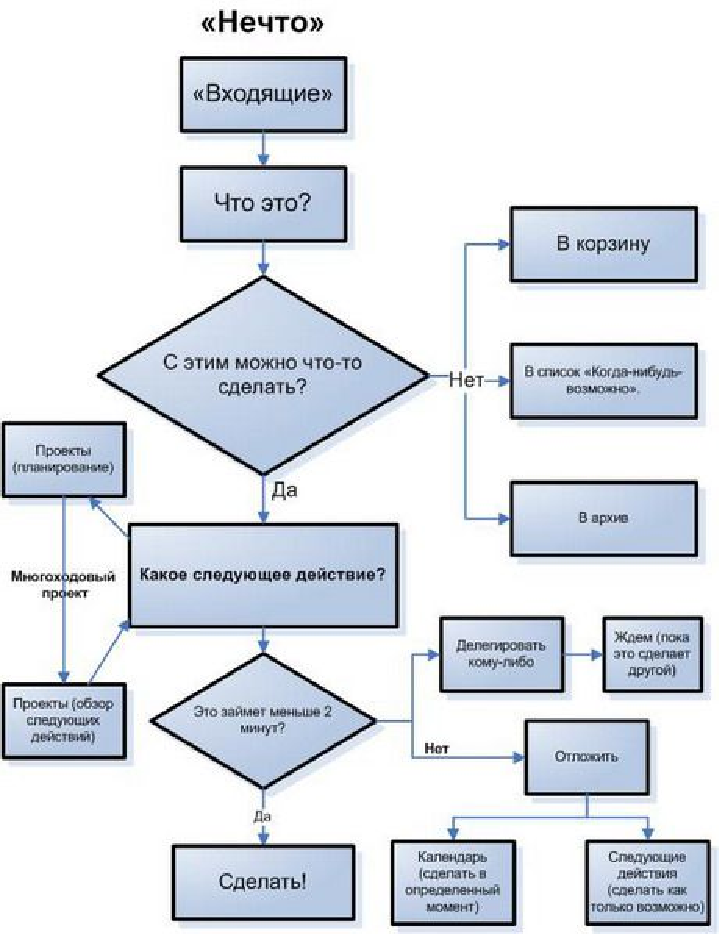
\includegraphics[width=0.5\textwidth]{GTDalgorithm.pdf}}
\end{frame}

\lecturenotes

Обработка корзины идёт строго по следующему алгоритму.
\begin{enumerate}
\item Начинаем с верхнего элемента корзины
\item Делаем один элемент за раз (при этом никогда ничего не возвращаем обратно)
  \begin{itemize}
  \item Если элемент требует действия:
    \begin{itemize}
    \item Делаем это (если на это требуется меньше двух-пяти минут), ИЛИ
    \item Делегируем это кому-нибудь, ИЛИ
    \item Откладываем это
    \end{itemize}
  \item Если элемент не требует действия:
    \begin{itemize}
    \item Оставляем это в справочной информации, ИЛИ
    \item Выбрасываем это, ИЛИ
    \item В список «когда-нибудь может быть»
    \end{itemize}
  \end{itemize}
\end{enumerate}
Если на действие требуется менее чем две-пять минут, это должно быть немедленно сделано. Двухминутное правило обусловлено тем примерным временем, которое нужно, чтобы формально отложить действие~\cite{GTDWikipedia}.

\begin{frame} \frametitle{Организация, Обзор, Действия}
  \begin{itemize}
  \item Организация: используются 4 вида списков: Следующие действия, Проекты, Отложенное, Когда-нибудь/может быть
  \item Обзор --- постоянно делать обзор списков
  \item Действия --- основная часть времени должно занимать именно дейсвтие, а не планирование
  \end{itemize}
\end{frame}

\lecturenotes

Организация
Для контроля за элементами, ожидающими внимания, Аллен советует использовать набор списков.
\begin{itemize}
\item Следующие действия --- По каждому элементу, требующему внимания, решите, что является следующим действием, которое может быть физически выполнено. Например, если имеется элемент «Написать проектный отчёт», следующее действие может быть таким: «Написать письмо Михаилу с предложением о встрече» или: «Позвонить Марине для того, чтобы узнать требования к отчёту». Хотя элемент может требовать довольно много шагов и действий, всегда будет что-то, что должно быть сделано сначала, и этот шаг должен быть описан в списке следующих действий. Предпочтительно, чтобы эти шаги были организованы по контексту, в котором они могут быть сделаны (например, «в офисе», «по телефону» или «в магазине»)
\item роекты --- Каждый разомкнутый цикл в жизни или работе, требующий больше чем одного физического действия для достижения цели, становится проектом. Проекты необходимо контролировать и периодически делать обзор, чтобы удостовериться, что с каждым проектом связано следующее действие, и, таким образом, проект будет продвигаться
\item Отложенное --- Когда действие было делегировано кому-то или когда ожидается некоторое внешнее событие, прежде чем проект может быть продвинут, это отслеживается в системе и периодически выясняется, требуется ли действие или нужно послать напоминание
\item Когда-нибудь/может быть -- Вещи, которые будут сделаны в некоторый момент, но не прямо сейчас. Например, «выучить китайский» или «устроить вечеринку в бассейне»
\end{itemize}

Календарь важен для контроля над встречами и поручениями; однако, Аллен рекомендует, чтобы календарь был зарезервирован только для тех вещей, которые должны быть сделаны в строго конкретный срок, или для встреч и поручений с заданным временем и местом. А дела должны быть зафиксированы в списках следующих действий, а не в календаре.

Последний ключевой организующий компонент GTD — система документов. Система документов должна быть лёгкой, простой и интересной. Даже единственный листок бумаги, если он нужен для справочной информации, должен получить свою собственную папку, если имеющиеся папки для него не подходят. Аллен предлагает одномерную, организованную в алфавитном порядке, систему хранения документов для того, чтобы быстро и просто восстанавливать необходимую информацию.

Обзор
Списки действий и напоминания будут мало полезны, если не делать обзор по крайней мере ежедневно, или настолько часто, насколько это возможно. Учитывая время, энергию и ресурсы, доступные в данный момент, нужно найти самую важную задачу, которая может быть сделана немедленно, и сделать её. Если Вы имеете привычку откладывать свои дела, всё закончится тем, что Вы будете делать простые задачи и избегать трудных. Для решения этой проблемы можно делать действия из списка один за другим, по аналогии с тем, как обрабатывается корзина. GTD требует, чтобы, по крайней мере, еженедельно проводился обзор по всем действиям, проектам и «отложенным» элементам для того, чтобы удостовериться, что любые новые задачи или предстоящие события введены в систему, и что всё актуально.

Действия
Любая организационная система бесполезна, если в ней слишком много времени тратится на организацию задач вместо физического их выполнения. Как утверждает Дэвид Аллен, если такую систему сделать простой для совершения необходимых действий, то человек будет менее склонен их откладывать или «перегружаться» слишком большим количеством «разомкнутых циклов»~\cite{GTDWikipedia}.

\section{Управление взаимодействием с другими сотрудниками}
\section{Инструменты организации деятельности отдельного разработчика}

\begin{thebibliography}{99}
\bibitem{TMHabr} \href{https://habrahabr.ru/post/259293/}{Тайм-менеджмент для разработчика / Хабрахабр}
\bibitem{TasksMedium} \href{https://medium.com/@skidanolegs/анализ-задачи-и-разбиение-задач-на-подзадачи-21b7865f387f}{Анализ задачи и разбиение задач на подзадачи – Oleg Skidan – Medium}
\bibitem{TasksHabr} \href{https://habrahabr.ru/post/111873/}{Разбиение на подзадачи: почему работает, и почему нет / Хабрахабр}
\bibitem{TMCodeProject} \href{https://www.codeproject.com/Articles/11502/Time-Management-Tips-for-Developers}{Time Management Tips for Developers - CodeProject}
\bibitem{TMSeimer} \href{https://lostechies.com/andrewsiemer/2016/01/04/developer-personal-time-management/]}{Developer personal time management | Andrew Seimer}
\bibitem{Pomidoro} \href{https://happydiva.ru/time-management/273-upravlenie-vremenem-metod-pomidora-pomodoro}{Управление временем: метод помидора (pomodoro)}
\bibitem{GTDWikipedia} \href{https://ru.wikipedia.org/wiki/Getting_Things_Done}{Getting Things Done — Википедия}
\end{thebibliography}

\end{document}

%%% Local Variables: 
%%% mode: TeX-pdf
%%% TeX-master: t
%%% End: 
